\documentclass[oneside]{book}

\usepackage[utf8]{inputenc}
\usepackage[T1]{fontenc}
\usepackage{ebgaramond}
\usepackage{graphicx}
\usepackage{fancyhdr}

\fancyhf{}
\fancyhead[L]{\scshape Jorge Luis Borges}
\fancyhead[R]{\scshape The Library Of Babel}
\fancyfoot[C]{\thepage}
\pagestyle{fancy}

\setlength\parindent{0em}
\setlength\parskip{1em}
\renewcommand\baselinestretch{1.15}
\graphicspath{ {./img/} }

\begin{document}

\begin{titlepage}
    \begin{center}
        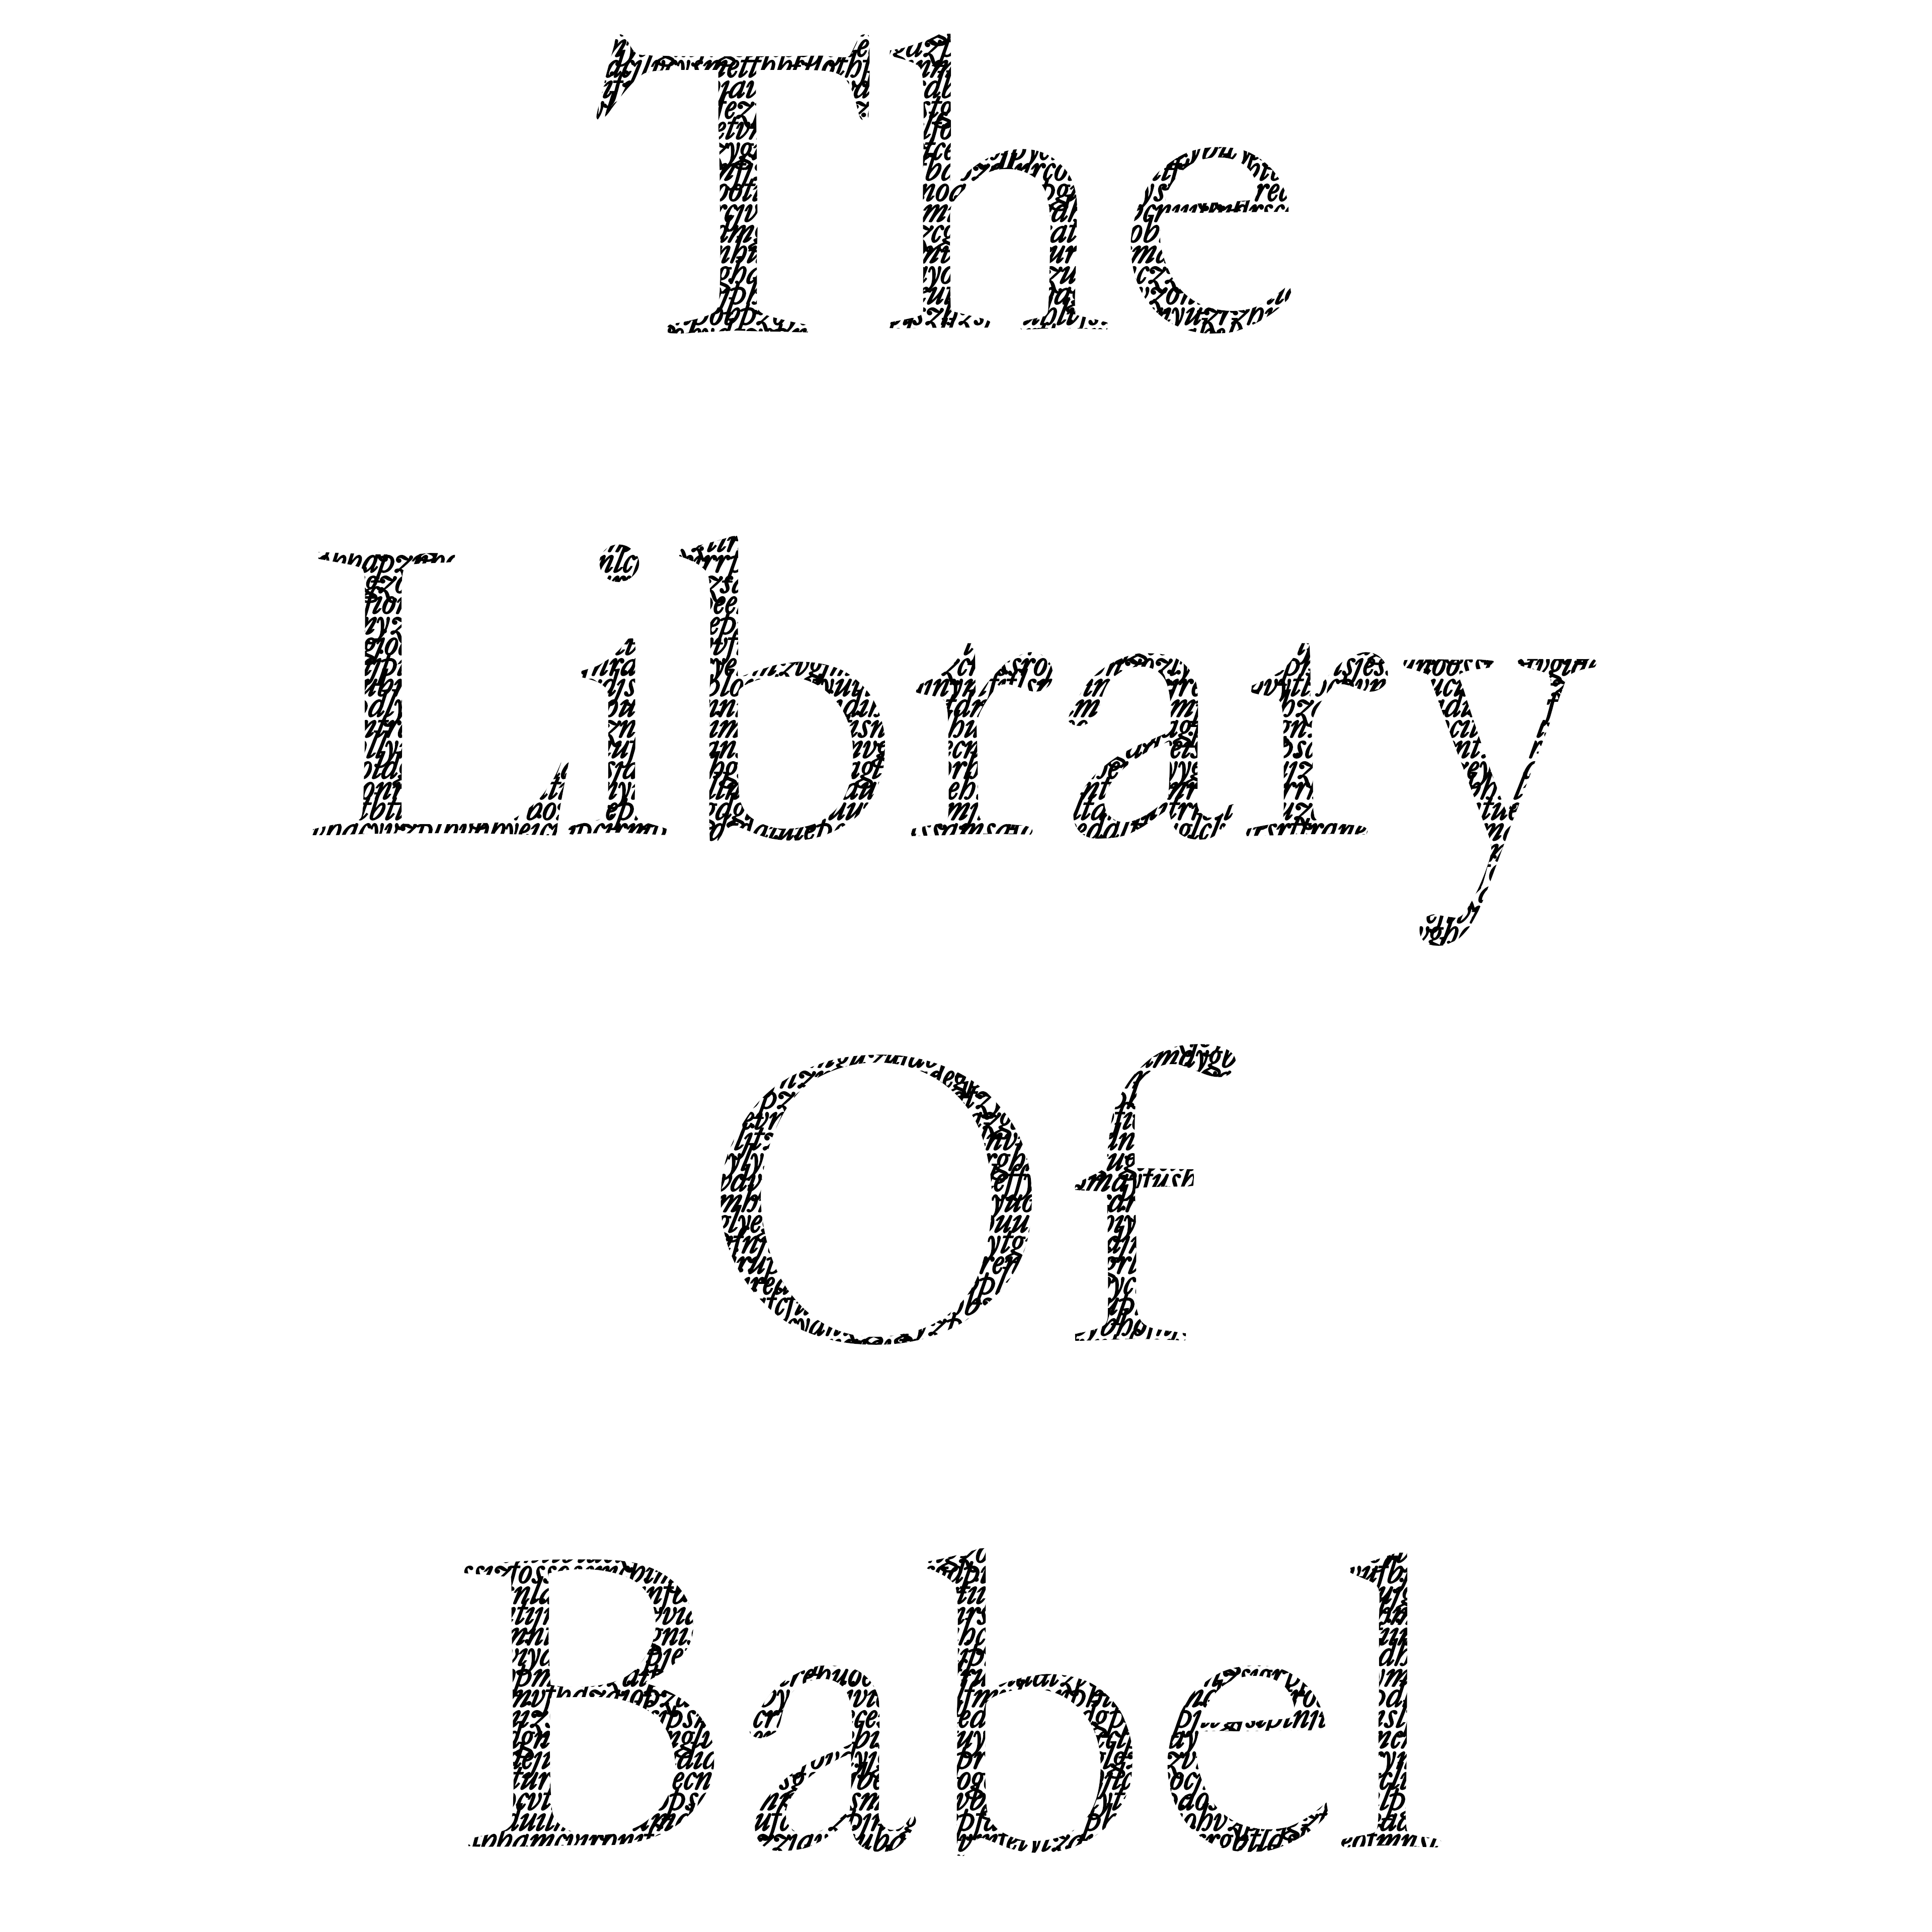
\includegraphics[width=\linewidth]{Title.png}

        \vfill

        \textsc{\Large Jorge Luis Borges}\par
        \textbf{1941}
    \end{center}
\end{titlepage}

\pagestyle{empty}
\begin{center}
    \leavevmode\vfill
    
    By this art you may contemplate the variations of the 23 letters\dots \par
    \vspace*{.8em}
    \hrule
    \textit{The Anatomy of Melancholy, part 2, sect. II, mem. IV}
    
    \vfill
\end{center}
\newpage

\pagestyle{fancy}
\setcounter{page}{1}

\bigskip

The universe (which others call the Library) is composed of an indefinite and perhaps infinite number of hexagonal galleries, with vast air shafts between, surrounded by very low railings. From any of the hexagons one can see, interminably, the upper and lower floors. The distribution of the galleries is invariable. Twenty shelves, five long shelves per side, cover all the sides except two; their height, which is the distance from floor to ceiling, scarcely exceeds that of a normal bookcase. One of the free sides leads to a narrow hallway which opens onto another gallery, identical to the first and to all the rest. To the left and right of the hallway there are two very small closets. In the first, one may sleep standing up; in the other, satisfy one's fecal necessities. Also through here passes a spiral stairway, which sinks abysmally and soars upwards to remote distances. In the hallway there is a mirror which faithfully duplicates all appearances. Men usually infer from this mirror that the Library is not infinite (if it were, why this illusory duplication?); I prefer to dream that its polished surfaces represent and promise the infinite\dots light is provided by some spherical fruit which bear the name of lamps. There are two, transversally placed, in each hexagon. The light they emit is insufficient, incessant.

Like all men of the Library, I have traveled in my youth; I have wandered in search of a book, perhaps the catalogue of catalogues; now that my eyes can hardly decipher what I write, I am preparing to die just a few leagues from the hexagon in which I was born. Once I am dead, there will be no lack of pious hands to throw me over the railing; my grave will be the fathomless air; my body will sink endlessly and decay and dissolve in the wind generated by the fall, which is infinite. I say that the Library is unending. The idealists argue that the hexagonal rooms are a necessary form of absolute space or, at least, of our intuition of space. They reason that a triangular or pentagonal room is inconceivable. (The mystics claim that their ecstasy reveals to them a circular chamber containing a great circular book, whose spine is continuous and which follows the complete circle of the walls; but their testimony is suspect; their words, obscure. This cyclical book is God.) Let it suffice now for me to repeat the classic dictum: \emph{The Library is a sphere whose exact center is any one of its hexagons and whose circumference is inaccessible.}

There are five shelves for each of the hexagon's walls; each shelf contains thirty-two books of uniform format; each book is of four hundred and ten pages; each page, of forty lines, each line, of some eighty letters which are black in color. There are also letters on the spine of each book; these letters do not indicate or prefigure what the pages will say. I know that this incoherence at one time seemed mysterious. Before summarizing the solution (whose discovery, in spite of its tragic projections, is perhaps the capital fact in history) I wish to recall a few axioms.

First: The Library exists \emph{ab aeterno}. This truth, whose immediate corollary is the future eternity of the world, cannot be placed in doubt by any reasonable mind. Man, the imperfect librarian, may be the product of chance or of malevolent demiurgi; the universe, with its elegant endowment of shelves, of enigmatical volumes, of inexhaustible stairways for the traveler and latrines for the seated librarian, can only be the work of a god. To perceive the distance between the divine and the human, it is enough to compare these crude wavering symbols which my fallible hand scrawls on the cover of a book, with the organic letters inside: punctual, delicate, perfectly black, inimitably symmetrical.

Second: \emph{The orthographical symbols are twenty-five in number.}\footnote{The original manuscript does not contain digits or capital letters. The punctuation has been limited to the comma and the period. These two signs, the space and the twenty-two letters of the alphabet are the twenty-five symbols considered sufficient by this unknown author. \emph{(Editor's note.)}} This finding made it possible, three hundred years ago, to formulate a general theory of the Library and solve satisfactorily the problem which no conjecture had deciphered: the formless and chaotic nature of almost all the books. One which my father saw in a hexagon on circuit fifteen ninety-four was made up of the letters MCV, perversely repeated from the first line to the last. Another (very much consulted in this area) is a mere labyrinth of letters, but the next-to-last page says \emph{Oh time thy pyramids}. This much is already known: for every sensible line of straightforward statement, there are leagues of senseless cacophonies, verbal jumbles and incoherences. (I know of an uncouth region whose librarians repudiate the vain and superstitious custom of finding a meaning in books and equate it with that of finding a meaning in dreams or in the chaotic lines of one's palm\dots they admit that the inventors of this writing imitated the twenty-five natural symbols, but maintain that this application is accidental and that the books signify nothing in themselves. This dictum, we shall see, is not entirely fallacious.)

For a long time it was believed that these impenetrable books corresponded to past or remote languages. It is true that the most ancient men, the first librarians, used a language quite different from the one we now speak; it is true that a few miles to the right the tongue is dialectical and that ninety floors farther up, it is incomprehensible. All this, I repeat, is true, but four hundred and ten pages of inalterable MCV's cannot correspond to any language, no matter how dialectical or rudimentary it may be. Some insinuated that each letter could influence the following one and that the value of MCV in the third line of page 71 was not the one the same series may have in another position on another page, but this vague thesis did not prevail. Others thought of cryptographs; generally, this conjecture has been accepted, though not in the sense in which it was formulated by its originators.

Five hundred years ago, the chief of an upper hexagon\footnote{Before, there was a man for every three hexagons. Suicide and pulmonary diseases have destroyed that proportion. A memory of unspeakable melancholy: at times I have traveled for many nights through corridors and along polished stairways without finding a single librarian.} came upon a book as confusing as the others, but which had nearly two pages of homogeneous lines. He showed his find to a wandering decoder who told him the lines were written in Portuguese; others said they were Yiddish. Within a century, the language was established: a Samoyedic Lithuanian dialect of Guarani, with classical Arabian inflections. The content was also deciphered: some notions of combinative analysis, illustrated with examples of variations with unlimited repetition. These examples made it possible for a librarian of genius to discover the fundamental law of the Library. This thinker observed that all the books, no matter how diverse they might be, are made up of the same elements: the space, the period, the comma, the twenty-two letters of the alphabet. He also alleged a fact which travelers have confirmed: \emph{In the vast Library there are no two identical books.} From these two incontrovertible premises he deduced that the Library is total and that its shelves register all the possible combinations of the twenty-odd orthographical symbols (a number which, though extremely vast, is not infinite): Everything: the minutely detailed history of the future, the archangels' autobiographies, the faithful catalogues of the Library, thousands and thousands of false catalogues, the demonstration of the fallacy of those catalogues, the demonstration of the fallacy of the true catalogue, the Gnostic gospel of Basilides, the commentary on that gospel, the commentary on the commentary on that gospel, the true story of your death, the translation of every book in all languages, the interpolations of every book in all books.

When it was proclaimed that the Library contained all books, the first impression was one of extravagant happiness. All men felt themselves to be the masters of an intact and secret treasure. There was no personal or world problem whose eloquent solution did not exist in some hexagon. The universe was justified, the universe suddenly usurped the unlimited dimensions of hope. At that time a great deal was said about the Vindications: books of apology and prophecy which vindicated for all time the acts of every man in the universe and retained prodigious arcana for his future. Thousands of the greedy abandoned their sweet native hexagons and rushed up the stairways, urged on by the vain intention of finding their Vindication. These pilgrims disputed in the narrow corridors, proferred dark curses, strangled each other on the divine stairways, flung the deceptive books into the air shafts, met their death cast down in a similar fashion by the inhabitants of remote regions. Others went mad\dots the Vindications exist (I have seen two which refer to persons of the future, to persons who are perhaps not imaginary) but the searchers did not remember that the possibility of a man's finding his Vindication, or some treacherous variation thereof, can be computed as zero.

At that time it was also hoped that a clarification of humanity's basic mysteries --- the origin of the Library and of time --- might be found. It is verisimilar that these grave mysteries could be explained in words: if the language of philosophers is not sufficient, the multiform Library will have produced the unprecedented language required, with its vocabularies and grammars. For four centuries now men have exhausted the hexagons\dots there are official searchers, \emph{inquisitors}. I have seen them in the performance of their function: they always arrive extremely tired from their journeys; they speak of a broken stairway which almost killed them; they talk with the librarian of galleries and stairs; sometimes they pick up the nearest volume and leaf through it, looking for infamous words.
Obviously, no one expects to discover anything.

As was natural, this inordinate hope was followed by an excessive depression. The certitude that some shelf in some hexagon held precious books and that these precious books were inaccessible, seemed almost intolerable. A blasphemous sect suggested that the searches should cease and that all men should juggle letters and symbols until they constructed, by an improbable gift of chance, these canonical books. The authorities were obliged to issue severe orders. The sect disappeared, but in my childhood I have seen old men who, for long periods of time, would hide in the latrines with some metal disks in a forbidden dice cup and feebly mimic the divine disorder.

Others, inversely, believed that it was fundamental to eliminate useless works. They invaded the hexagons, showed credentials which were not always false, leafed through a volume with displeasure and condemned whole shelves: their hygienic, ascetic furor caused the senseless perdition of millions of books. Their name is execrated, but those who deplore the ``treasures'' destroyed by this frenzy neglect two notable facts. One: the Library is so enormous that any reduction of human origin is infinitesimal. The other: every copy is unique, irreplaceable, but (since the Library is total) there are always several hundred thousand imperfect facsimiles: works which differ only in a letter or a comma. Counter to general opinion, I venture to suppose that the consequences of the Purifiers' depredations have been exaggerated by the horror these fanatics produced. They were urged on by the delirium of trying to reach the books in the Crimson Hexagon: books whose format is smaller than usual, all-powerful, illustrated and magical.

We also know of another superstition of that time: that of the Man of the Book. On some shelf in some hexagon (men reasoned) there must exist a book which is the formula and perfect compendium of \emph{all the rest}: some librarian has gone through it and he is analogous to a god. In the language of this zone vestiges of this remote functionary's cult still persist. Many wandered in search of Him. For a century they have exhausted in vain the most varied areas. How could one locate the venerated and secret hexagon which housed Him? Someone proposed a regressive method: To locate book A, consult first book B which indicates A's position; to locate book B, consult first a book C, and so on to infinity\dots in adventures such as these, I have squandered and wasted my years. It does not seem unlikely to me that there is a total book on some shelf of the universe\footnote{I repeat: it suffices that a book be possible for it to exist. Only the impossible is excluded. For example: no book can be a ladder, although no doubt there are books which discuss and negate and demonstrate this possibility and others whose structure corresponds to that of a ladder.}; I pray to the unknown gods that a man --- just one, even though it were thousands of years ago! --- may have examined and read it. If honor and wisdom and happiness are not for me, let them be for others. Let heaven exist, though my place be in hell. Let me be outraged and annihilated, but for one instant, in one being, let Your enormous Library be justified. The impious maintain that nonsense is normal in the Library and that the reasonable (and even humble and pure coherence) is an almost miraculous exception. They speak (I know) of the ``feverish Library whose chance volumes are constantly in danger of changing into others and affirm, negate and confuse everything like a delirious divinity.'' These words, which not only denounce the disorder but exemplify it as well, notoriously prove their authors' abominable taste and desperate ignorance. In truth, the Library includes all verbal structures, all variations permitted by the twenty-five orthographical symbols, but not a single example of absolute nonsense. It is useless to observe that the best volume of the many hexagons under my administration is entitled \emph{The Combed Thunderclap} and another \emph{The Plaster Cramp} and another \emph{Axaxaxas mlö}. These phrases, at first glance incoherent, can no doubt be justified in a cryptographical or allegorical manner; such a justification is verbal and,  ex hypothesi, already figures in the Library. I cannot combine some characters

\begin{quote}\itshape
    dhcmrlchtdj
\end{quote}

which the divine Library has not foreseen and which in one of its secret tongues do not contain a terrible meaning. No one can articulate a syllable which is not filled with tenderness and fear, which is not, in one of these languages, the powerful name of a god. To speak is to fall into tautology. This wordy and useless epistle already exists in one of the thirty volumes of the five shelves of one of the innumerable hexagons --- and its refutation as well. (An $n$ number of possible languages use the same vocabulary; in some of them, the symbol \textit{library} allows the correct definition \textit{a ubiquitous and lasting system of hexagonal galleries}, but \textit{library} is \textit{bread} or \textit{pyramid} or anything else, and these seven words which define it have another value. You who read me, are You sure of understanding my language?)

The methodical task of writing distracts me from the present state of men. The certitude that everything has been written negates us or turns us into phantoms. I know of districts in which the young men prostrate themselves before books and kiss their pages in a barbarous manner, but they do not know how to decipher a single letter. Epidemics, heretical conflicts, peregrinations which inevitably degenerate into banditry, have decimated the population. I believe I have mentioned suicides, more and more frequent with the years. Perhaps my old age and fearfulness deceive me, but I suspect that the human species --- the unique species --- is about to be extinguished, but the Library will endure: illuminated, solitary, infinite, perfectly motionless, equipped with precious volumes, useless, incorruptible, secret.

I have just written the word ``infinite.'' I have not interpolated this adjective out of rhetorical habit; I say that it is not illogical to think that the world is infinite. Those who judge it to be limited postulate that in remote places the corridors and stairways and hexagons can conceivably come to an end --- which is absurd. Those who imagine it to be without limit forget that the possible number of books does have such a limit. I venture to suggest this solution to the ancient problem:  The Library is unlimited and cyclical. If an eternal traveler were to cross it in any direction, after centuries he would see that the same volumes were repeated in the same disorder (which, thus repeated, would be an order: the Order). My solitude is gladdened by this elegant hope\footnote{Letizia Álvarez de Toledo has observed that this vast Library is useless: rigorously speaking, \emph{a single volume} would be sufficient, a volume of ordinary format, printed in nine or ten point type, containing an infinite number if infinitely thin leaves. (In the early seventeenth century, Cavalieri said that all solid bodies are the superimposition of an infinite number of planes.) The handling of this silky vade mecum would not be convenient: each apparent page would unfold into other analogous ones; the inconceivable middle page would have no reverse.}.

\end{document}
